\chapter*{Appendix} \label{sec:appendix}

\section*{Large Language Models as Recommenders} \label{sec:large-language-models-as-recommenders}

The rise of modern \ac{LLMs} such as GPT4 \cite{OpenAIGPT4Technical2023} has revolutionized the field of \ac{NLP}, demonstrating impressive capabilities in a variety of tasks.
This section provides an overview of the potential of \ac{LLMs} in the context of recommender systems.
In recent years, several studies have explored using \ac{LLMs} in recommendation tasks, showing promising results \cite{ZhangLanguageModels2021, HouLargeLanguage2023, LiGPT4RecGenerative2023}.
Although this thesis does not utilize generative \ac{LLMs}, this discussion serves to contextualize the broader landscape of advancements in the field and to provide insights into potential future directions.

Li et al. \cite{LiGPT4RecGenerative2023} introduced a novel generative framework for personalized recommendations. Their model, inspired by search engines and built on Transformer models, views items as queries. It then adopts a generative method to estimate the conditional probability of a user's next action based on their history. This method effectively captures the content information of items, interprets user interests, and adapts to changing item inventories.

Liu et al. \cite{LiuChatGPTGood2023} examined the potential of ChatGPT\footnote{\url{https://openai.com/blog/chatgpt}} as a general-purpose recommender model. They framed recommendation tasks as a conversation between the user and the system, leveraging ChatGPT to generate recommendations from the user's input. Their findings indicate that ChatGPT is comparable to traditional recommendation methods for several tasks and even excels in tasks that require a deeper understanding of user preferences.

Despite the promising potential of \ac{LLMs}, their use in recommender systems presents challenges. These encompass the high computational cost of training and deploying such models, the need for vast amounts of data for pre-training, and the model's limited interpretability, which hampers understanding and justification of their recommendations \cite{LinHowCan2023, LiuPretrainPrompt2023}. Moreover, Liu et al. \cite{LiuChatGPTGood2023} highlight that \ac{LLMs} often recommend popular items, leading to a lack of diversity and novelty in the recommendations. Finally, the way users phrase their input greatly influences the recommendations, causing inconsistent outcomes \cite{ZhangLanguageModels2021}.


\section*{Hybrid Recommender Evaluation} \label{sec:hybrid-recommender-evaluation}

\begin{figure}[htb!]
    \centering
    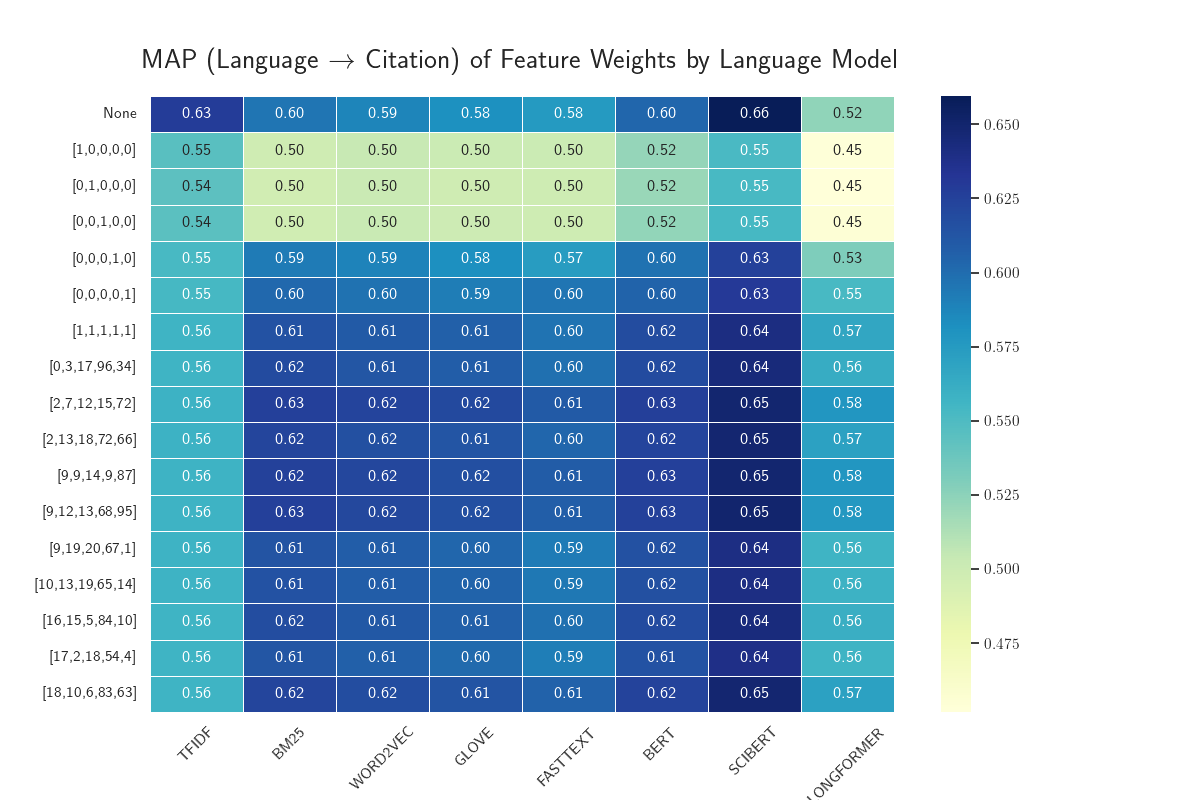
\includegraphics[width=\textwidth]{plots/language_models_feature_weights_heatmap_l_to_c.png}
    \caption[Performance Evaluation of the \acl{L2C} Hybrid Recommender]{Performance Evaluation of the \ac{L2C} Hybrid Recommender using different feature weights and language models. Darker colors correspond to higher \ac{MAP} values.
        The first row displays the \ac{MAP} values for the Language Recommender candidates before re-ranking. Subsequent rows show \ac{MAP} values for each language model after being re-ranked by the Citation Recommender with the corresponding weight vector.
        The trend concerning which language models improve or degrade due to re-ranking is consistent with the results in \Cref{fig:hybridization-strategies-by-language-model}.
        With the exception of TF-IDF, weight vectors with zero weight for co-citation analysis and bibliographic coupling score notably underperform.
        Compared to the feature weights ranking for candidate selection (\Cref{fig:feature-weights-evaluation}), the unit weight vectors $[0, 0, 0, 1, 0]$ and $[0, 0, 0, 0, 1]$ perform worse relative mixed non-zero weight vectors.
        This observation is consistent across all language models, except for TF-IDF.}
    \label{fig:language-models-feature-weights-heatmap-l2c}
\end{figure}
